\documentclass[12pt, letterpaper]{article}

\usepackage{graphicx}
\usepackage{parskip} % Disabling paragraph index as it does not fit maths
\usepackage{hyperref} % Usable menu and references
\usepackage{amssymb} % Used to show sets of sumbers, like the real numbers
\usepackage{amsmath} % Used for column vectors
\usepackage{xargs} % Used for multiple deafult command values
\usepackage{pgfplots} % Used for plots

\graphicspath{{images}}

\newcommand{\R}{\mathbb{R}}
\newcommand{\C}{\mathbb{C}}
\newcommand{\Q}{\mathbb{Q}}
\newcommand{\Z}{\mathbb{Z}}
\newcommand{\slv}{\mathfrak{sl} (3, \C)}

\newcommandx{\rang}[2][1=\alpha,2=\beta]{\frac{2(#2, #1)}{(#1, #1)}}

\title{Project Prereading}
\author{Arkadiusz Naks}
\date{2024}

\begin{document}

\tableofcontents
\newpage

\begin{section}{Root Systems by Laval}

  \(\slv\) is the vector space containing all \(3 \times 3\)
  matricies M s.t.\ the diagonal adds up to 0. This is a vector space with
  baisis \(\{H_{1}, H_{2}, M_{i,j}\}\) where \(i \neq j \in \{1, 2, 3\}\). \\
  \(M_{1,2} =
  \begin{pmatrix}
    0 && 1 && 0 \\
    0 && 0 && 0 \\
    0 && 0 && 0 \\
  \end{pmatrix}\), \(H_{1} =
  \begin{pmatrix}
    1 && 0 && 0 \\
    0 && 0 && 0 \\
    0 && 0 && -1 \\
  \end{pmatrix}\) and \(H_{2} =
  \begin{pmatrix}
    1 && 0 && 0 \\
    0 && -1 && 0 \\
    0 && 0 && 0 \\
  \end{pmatrix}\)

  For \(X, Y \in \slv\) \([X, Y] = XY -YX\). This operation is closed on
  \(\slv\) and together they form a Lie algebra (expand later). \\
  A Cartan subalgebra of \(\slv\), denoted \(\mathfrak{h}\) is a subspace of
  all diagonal matricies. For any element \(H \in \mathfrak{h}\)
  \([H, H_{i}] = 0\) and \([H, M_{i, j}] = (\theta_{i} - \theta_{j})M_{i,j}\).

  \begin{subsection}{Root Systems}

    As \(\theta_{3} = -\theta_{1} - \theta_{2}\) all elements
    \(\theta_{i} - \theta_{j}\) can be writen in terms of \(\theta_{1}\) and
    \(\theta_{2}\). When graphing all these points on a graph with axis
    \(\frac{2 \pi}{3}\), they form a regular hexagon. Considering these points
    as vecotrs in \(\R^{2}\) with all of them being in a set \(\Phi\).
    Although \(\Phi\) is not a subspace as it does not contain the zero vector
    although it clearly spans \(\R^{2}\). Below is a plot with all the vecotrs:

    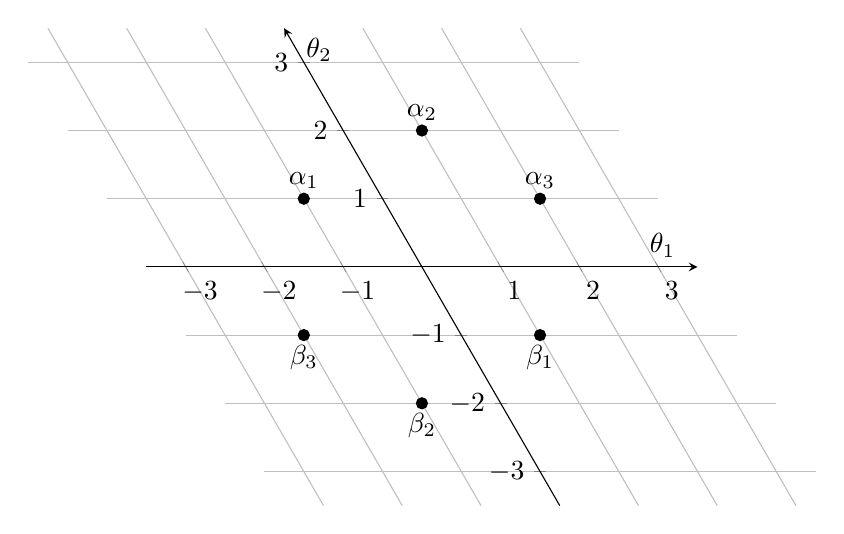
\begin{tikzpicture}[thick]
      \begin{axis}[
        axis lines = center,
        xlabel = {\(\theta_{1}\)},
        ylabel = {\(\theta_{2}\)},
        x={(1cm,0cm)}, y={(-0.5cm,0.86602540378cm)},
        grid=major,
        xmin=-3.5 , xmax=3.5,
        ymin=-3.5 ,ymax=3.5,
        ]

        \addplot[mark=*] coordinates {(-1,1)} node[above,pos=1]
        {\(\alpha_{1}\)};
        \addplot[mark=*] coordinates {(1,2)} node[above,pos=1]
        {\(\alpha_{2}\)};
        \addplot[mark=*] coordinates {(2,1)} node[above,pos=1]
        {\(\alpha_{3}\)};

        \addplot[mark=*] coordinates {(1,-1)} node[below,pos=1]
        {\(\beta_{1}\)};
        \addplot[mark=*] coordinates {(-1,-2)} node[below,pos=1]
        {\(\beta_{2}\)};
        \addplot[mark=*] coordinates {(-2,-1)} node[below,pos=1]
        {\(\beta_{3}\)};

      \end{axis}
    \end{tikzpicture}


    As seen in the plot, \(\alpha_{i} = -\beta_{i}\). This means that
    \(\forall \alpha \in \Phi \Rightarrow -\alpha \in \Phi\). \(\Phi\) is also
    unchanded by any reflection in a line orthogonal to one of its vectors.
    Lastly any vector \(\alpha\) projected to another vecotr \(\beta\), the
    projection is equal to a half integer multiple of \(\beta\).

    \(\Phi\) is a root system called \(A_{2}\).

  \end{subsection}

  \begin{subsection}{Root Systems Formally}

    \begin{subsubsection}{Setup Axioms}

      Let V be a finite dimensional real inner product space over \(\R\) with
      the inner product \((,) : V \times V \to \R\). If V is 2D, then a
      reflection in V is a linear transformation that fixes a line in the
      vecotr space and sends any vector orthogonal to that line to its
      negative. For higher dimensions, the line is replaced by a
      \textbf{hyperplane} which is subspace of V with one less dimension than V.

      Formally for any \(\alpha \in V\) \(\sigma_{\alpha}\) represents a
      reflaction in the hyperplane
      \(P_{\alpha} = \{\beta \in V : (\beta, \alpha) = 0\}\). Then
      \[\sigma_{\alpha}(\beta) = \beta - \rang \alpha.\]
      For simplicity define \(\langle \beta, \alpha \rangle = \rang\). This is
      also euqal to \(2 \frac{|\beta|}{|\alpha|} \cos \theta\).
      Reflections preserve the lengths of and angles between vectors. Formally
      \((\beta, \gamma) = (\sigma_{\alpha}(\beta), \sigma_{\beta}(\gamma))\).
      Also \(\beta = \sigma_{\alpha}(\sigma_{\alpha}(\beta))\). Clearly this
      means that reflections are injective.

    \end{subsubsection}

    \begin{subsubsection}{Properties}

      In general, all root systems \(\Phi\) have to follow the same rules as
      \(A_{2}\), which formally are
      \begin{itemize}
        \item \(\Phi\) is finite set that spans V
        \item \(0 \notin \Phi\)
        \item If \(\alpha \in \Phi \Rightarrow -\alpha \in \Phi\) and
              \(n \alpha \notin \Phi\) for \(n \neq 1,-1\)
        \item \(\alpha \in \Phi \Rightarrow \sigma_{\alpha}(\Phi) = \Phi\)
        \item If \(\alpha, \beta \in \Phi \Rightarrow \rang \in \Z\)
      \end{itemize}

      All elements of such system are called roots. Sometimes the third point
      is omitted and the above definition is called a \textbf{reduced} root
      system. Similarly sometimes the fith point is ommited and the above one
      is called \textbf{crystallographic} root system.

    \end{subsubsection}

    \begin{subsubsection}{Positive Systems}

      For \(\mathfrak{B} = \{v_{i}\}\) a basis of V, any root
      \(\alpha \in \Phi\) is equal to \(\sum^{n}_{0} \lambda_{i} v_{i}\) for
      \(\lambda_{i} \in \R\). Then \(\alpha\) is positive with respect to
      \(\mathfrak{B}\) if \(0 < \lambda_{k}\) with k the smallest non zero
      index. Otherwise \(\alpha\) is negative. \\
      A positive system, denoted \(\Phi^{+}\), contains all positive
      \(\alpha\) with respect to some basis.

      For any root system
      \begin{itemize}
        \item \(\Phi^{+} \cap \Phi^{-} = \emptyset\)
        \item \(\Phi^{+} \cup \Phi^{-} = \Phi\)
        \item \(\Phi^{-}  = -\Phi^{+}\)
      \end{itemize}

      Every positive system contains a unique simple system.

    \end{subsubsection}

    \begin{subsubsection}{Simple Systems}

      To construct a 2D root system, only two vectors \(\alpha\) and \(\beta\)
      are needed while the rest can be obtained by taking the reflections in
      \(P_{\alpha}\) and \(P_{\beta}\). A simple system, also sometimes called a
      base, of a root system is \(\Delta \subset \Phi\) s.t.\ it is a basis and
      each element can be obtained by same sign coefficients for all the basis
      elements.

      If a simple system exists, there exists a unique positive system
      containing it.

      Although positive and negatie systems are not invariant under reflections,
      if \(\Delta \subset \Phi^{+}\) then for every \(\alpha \in \Delta\)
      \(\sigma_{\alpha}(\Phi^{+} \backslash \{\alpha\}) =
      \Phi^{+} \backslash \{\alpha\}\)

      For all \(\alpha \neq \beta \in \Delta\) \((\alpha, \beta) \leq 0\).

      For \(\beta \in \Phi\) if \(\beta = \sum_{\alpha \in \Delta}
      \lambda_{\alpha} \alpha\), the height of \(\beta\) is defined as
      \(ht(\beta) = \sum_{\alpha \in \Delta} \lambda_{\alpha}\).

    \end{subsubsection}

  \end{subsection}

  \begin{subsection}{The Weyl Group}

    The Weyl group, denoted \(W\), is a subgroup of \(GL_{n}(\R)\) which is
    generated by \(\sigma_{\alpha}\) \(\forall \alpha \in \Phi\). If
    \(w \in W\) and \(\alpha \in \Phi\) then
    \(w \sigma_{\alpha} w^{-1} = \sigma_{wa}\). W is always generated by
    \(\sigma_{\alpha}\) \(\forall \alpha \in \Delta\).

    For every \(\beta \in \Phi \;\; \exists w \in W\) s.t.\
    \(w \beta \in \Delta\).

  \end{subsection}

  \begin{subsection}{Classification}

    A root system is irreducible if it cannot be partitioned into an union of
    two proper subsets \(\Phi = \Phi_{1} \cup \Phi_{2}\) s.t.\
    \((\alpha, \beta) = 0\) \(\forall \alpha \in \Phi_{1},
    \beta \in \Phi_{2}\). It is enough to konw the angles and lenghts of all
    roots in the simple system to create the entire root system (by first
    generating its Weyl group). This information can be encoded into a graph
    much easier than multidimentional root systems.

    \begin{subsubsection}{Coxeter Graphs}

      For \(\Delta = \{\alpha_{1}, \dots, \alpha_{n}\}\), a Coxeter graph of
      \(\Phi\) with respect to \(\Delta\) contains n verticies labeled from 1
      to n with the ith vertex joined to the jth vertex by \(\langle
      \alpha_{i}, \alpha_{j} \rangle \langle \alpha_{j}, \alpha_{i} \rangle\)
      edges for \(i \neq j\). If \(\Phi\) and \(\Phi'\) have the same Coxeter
      graph, they are isomorphic. This means the graph is independent of
      \(\Delta\).

      The angles can be deduced as \(\langle \alpha_{i}, \alpha_{j} \rangle
      \langle \alpha_{j}, \alpha_{i} \rangle = 4 \cos^{2}(\theta)\).

      \(\Phi\) is irreducible \textbf{if and only if} its Coxeter graph is
      connected.

    \end{subsubsection}

    \begin{subsubsection}{Dynkin Diagram}

      The problem with Coxeter graphs is they dont describe lenghts of simple
      roots. In a Dynkin diagrams, there is an arrow on one of every multiedge
      pointing towards the \textbf{shorter} of the two roots (as for single
      edge the roots are same lenght).

    \end{subsubsection}

    \begin{subsubsection}{Admissable Set}

      A set of vectors \(\mathfrak{u} = \{\epsilon_{1.}, \dots,
      \epsilon_{n}\}\) is called admissible if the vectors are linearly
      independet and unit s.t.\ \(\epsilon_{i}, \epsilon_{j} \leq 0\) and
      \(4(\epsilon_{i}, \epsilon_{j}){}^{2} = 0,1,2,3\) for \(i \neq j\). To
      \(\mathfrak{u}\) we attach a graph \(\Gamma\) with n vertices labelled
      fom 1 to n with i and j connected
      \(4(\epsilon_{i}, \epsilon_{j}){}^{2}\) edges.\\
      For any simple set, the roots divided by their lenghts (to make them
      unit) form an admissable set.

      Some properties of \(\mathfrak{u}\):
      \begin{itemize}
        \item For any \(\mathfrak{u}' \subset \mathfrak{u}\) non-empty,
              \(\mathfrak{u}'\) is also admissable with the same graph with
              omittion
              of verticies missing in \(\mathfrak{u}'\).
        \item \(0 < n + 2 \sum^{n}_{i < j} (\epsilon_{i}, \epsilon_{j})\)
        \item The number of pairs of verticies connected by at least one edge
              is strictly less than n
      \end{itemize}

      This implies \(\Gamma\) contains no cycles.

      Let \(S \subset \mathfrak{u}\) s.t.\ it forms a simple chain in
      \(\Gamma\). Then defining \(\epsilon = sum(S)\) \(\mathfrak{u}' =
      (\mathfrak{u} \backslash S) \cup \{\epsilon\}\). This is because the
      graph for \(\mathfrak{u}'\) can be obtained by shrinking the simple
      chain in \(\Gamma\) to a single point.\\
      \emph{No more than three edges can occur at any given vertice of
        \(\Gamma\)}. This is a very important property when identifying
      graphis which cannot come from admissable set.

      Some properties of \(\Gamma\) a connected graph associated to an
      admissable set
      \begin{itemize}
        \item If it has a triple edge then it is a \(G_{2}\) graph
        \item Can have at most one double edge
        \item Can have at most one branch point
        \item Cannot contain both a double edge and a branch point
        \item If it contains only single endges and no branch points, it is a
              simple chain
      \end{itemize}

    \end{subsubsection}

    \begin{subsubsection}{Classification Theorem}

      If \(\Phi\) is an irreducible rot system with \(dim V =
      | \Delta | = n\), then its Dynkin diagram is one of the following
      \begin{itemize}
        \item \(A_{n}, n > 0\) which is a simple chain
        \item \(B_{n}, n > 1\) which is a simple chain with a double edge at
              the end poining away from the chain
        \item \(C_{n}, n > 2\) which is a simple chain with a double edge at
              the end poining towards the chain
        \item \(D_{n}, n > 3\) which is a simple chain with a branch point at
              the end
        \item \(E_{6}\) which is \(A_{5}\) with a single enge from the middle
        \item \(E_{7}\) which is \(E_{6}\) with one more vertex at the end
        \item \(E_{8}\) which is \(E_{6}\) with two more vertecies at the end
        \item \(F_{4}\) which is vertex, edge, vertex, double edge, vertex,
              edge, vertex
        \item \(G_{2}\) two verticies with a triple edge
      \end{itemize}

    \end{subsubsection}

  \end{subsection}

  \begin{subsection}{Lie Algebra Definision}

    Let \(\mathfrak{g}\) be a vector space with a map \([,]: \mathfrak{g}
    \times \mathfrak{g} \to \mathfrak{g}\) called the Lie bracket s.t.\ for
    \(x, y, z \in \mathfrak{g}\)
    \begin{itemize}
      \item The map is bilinear
      \item \([x, y] = -[y, x]\) (skew-symmetric)
      \item \([x, [y, z]] + [y, [z, x]] + [z, [x, y]] = 0\) (Jacobi identity)
    \end{itemize}
    Then \(\mathfrak{g}\) is called a Lie algebra.

    Non associative ring structure.

    \emph{Any Lie algebra is a complex inner product space.}

    \begin{subsubsection}{Ideals}

      For I a subspace of \(\mathfrak{g}\), I is called an ideal of
      \(\mathfrak{g}\) if \([x, y] \in I \;\; \forall x \in I,\; y\in
      \mathfrak{g}\). This definision is analogous to ideals in rings. \\
      A proper ideal is not equall to \(\mathfrak{g}\). If \(I = \{0\}\), it is
      called the trivial ideal.

    \end{subsubsection}

    \begin{subsubsection}{Semisimple Lie}

      A Lie algebra is called simple if \(dim \; \mathfrak{g} > 1\) and it
      contains no \textbf{proper, non-trivial} ideals.

      A Lie algebra is semisimple if it is the direct product of simple Lie
      algebras.

      A root system can always be retrived from a \textbf{semisimple} lie
      algebra. As all root systems can be classified, all semisimple lie
      algebras can be classified.

    \end{subsubsection}

    \begin{subsubsection}{Subalgebras}

      For \(\mathfrak{g}\) a matrix Lie algebra, \(\mathfrak{h}\) is a
      \textbf{toral} subalgebra iff all of its elements are diagonalizable. It
      is maximal if it is not contained in any other toral subalgebra of
      \(\mathfrak{g}\), and then it is also called a \textbf{Cartan} subalgebra.

      Every finite dimensinal complex Lie algebra contains a Cartan subalgebra.

    \end{subsubsection}

  \end{subsection}

  \begin{subsection}{Lie Root Systems}

    \begin{subsubsection}{Forms}

      Adjoint form/representation is a map \(ad_{x} : \mathfrak{g} \times
      \mathfrak{g} \to \C\) for some \(x \in \mathfrak{g}\) where \(ad_{x}(y)
      = [x, y]\). \emph{its probably actually just
        \(\mathfrak{g} \to \mathfrak{g}\)}.

      A map \(K(,): \mathfrak{g} \times \mathfrak{g} \to \C\) where \(K(x, y) =
      tr(ad_{x} \cdot ad_{y})\) s.t.\ this map is conjugate summetric, linear in
      the first argument and positive definite, implying that it is a complex
      inner product. It is called the Killing form on \(\mathfrak{g}\).

    \end{subsubsection}

    \begin{subsubsection}{Root Space}

      Define \(\mathfrak{h}^{*} = \{\phi : \mathfrak{h} \to \C : \phi\) is
      linear \(\}\). Then for \(\mathfrak{g}\) a semisimple finite dimensional
      complex Lie algebra and \(\mathfrak{h}\) its Cartan subalgebra,
      \(\mathfrak{g}\) can be \textbf{decomposed} to
      \(\oplus \mathfrak{g}_{\alpha}\)
      where \[\mathfrak{g}_{\alpha} = \{x \in \mathfrak{g} :[h, x] =
        \alpha(h)x, h \in \mathfrak{h}, \alpha \in \mathfrak{h}^{*}\}.\]
      This is called the \textbf{root space decomposition} of \(\mathfrak{g}\)
      and non-zero alphas are called \textbf{roots}. \\

      \(\mathfrak{h}^{*}\) is called the \textbf{dual space} of \(\mathfrak{h}\)
      and is an inner product space with the inner product
      \(K^{*}(\alpha, \beta) = K(t_{\alpha}, t_{\beta})\) where \(t_{\phi}\) is
      the unique element s.t.\ \(\phi(h) = K(t_{\phi}, h) \;\;
      \forall h \in \mathfrak{h}\). \(K^{*}(,)\) is called the \textbf{dual
        Killing form} of \(\mathfrak{h}^{*}\).

    \end{subsubsection}

    \begin{subsubsection}{The Link}

      The subset \(\{\alpha \in \mathfrak{h}^{*} :
      \mathfrak{g}_{\alpha} \neq 0\}\) is a root system with respect to the dual
      Killing form. It is called the root system of \(\mathfrak{g}\) with
      respect to \(\mathfrak{h}\). \\
      If two roots systems of two Lie algebras are isomorphic, then so are the
      algebras. Every root system has an root system of a Lie algebra isomorphic
      to itself. \\
      This means that classifying root systems equivelant to classifying
      semisimple Lie algebras.

    \end{subsubsection}

  \end{subsection}

\end{section}

\begin{section}{Wolfam}

  \begin{subsection}{Cartan Matricies}

    A \textbf{Cartan matrix} is a square matrix \(A_{i,j}\) s.t.\
    \begin{itemize}
      \item \(A_{i,j} \in \{-3, -2. -1, 0\}\) for \(i \neq j\)
      \item \(A_{i,i} = 2\)
      \item \(A_{i,j} = 0 \Rightarrow A_{j,i} = 0\)
      \item Tthere exists a diagonal matrix D s.t.\ \(DAD^{-1}\) is
            \textbf{symmetric} and has \textbf{positive definite quadratic form}
            (all its eigenvalues are positive)
    \end{itemize}

    Such matrix can be associated to a semisimple Lie algebra \(\mathfrak{g}\).
    If \(A\) is \(k \times k\), then k is also the rank of \(\mathfrak{g}\). In
    this correspondence, \[\langle \alpha_{i}, \alpha_{j} \rangle = A_{i,j}.\]
    Expand on what is \(\alpha_{i}\).

  \end{subsection}

\end{section}

\begin{section}{Book by B.C. Hall}

  \begin{subsection}{Lie Groups of Matricies}

    A \textbf{matrix Lie group} is a subgroup G of \(GL_{n}(\C)\) with a
    property that any sequnece \(A_{m} \in G\) converges to A then either
    \(A \in G\) or \(A \notin GL_{n}(\C)\). This condition is called being
    closed in GL. This means Lie groups are \textbf{closed subgroups}. Most
    Lie groups are \textbf{closed} in \(M_{n}(\C)\), meaning any sequence
    converging to A means that \(A \in G\).

    \begin{subsubsection}{Compactness}

      A Lie group is \textbf{compact} if
      \begin{itemize}
        \item It is closed in \(M_{n}\)
        \item All entries in every \(A \in G\) have bounded absolute value
      \end{itemize}
      This is equivelant to G begin \textbf{closed} and \textbf{bounded} subset
      of \(\C^{n^{2}}\).

    \end{subsubsection}

    \begin{subsubsection}{Connectedness}

      G is connected if for any \(A, B \in G\) \(\exists A(t) \in G: \;
      a \leq t \leq b\) s.t.\ \(A(a) = A\) and \(A(b) = B\) and \(A(t)\)
      continuous.

      A matrix Lie group G that is not connected, it can be decomposed
      \textit{uniquely} as a union of connected \textbf{components}. The
      component containing the identity is a subgoup of G.

      G is said to be \textbf{simply connected} if it is connected and for any
      \(A(t); \; 0 \leq t \leq 1\) s.t.\ \(A(0) = A(1)\), \(\exists A(s, t)\)
      satisfying
      \begin{itemize}
        \item It is continues
        \item \(A(s, 0) = A(s, 1)\) it is a loop for all s
        \item \(A(0, t) = A(t)\)
        \item \(A(1, t) = A(1, 0)\) it is a point for \(s = 1\)
      \end{itemize}

      If a matrix Lie group G is simply connected, there is a natural one to one
      correspondence between the representations of G and the representations of
      its Lie algebra. Also G begin simply connected iff its \textbf{fundamental
        group} is \(\{1\}\).

    \end{subsubsection}

    \begin{subsubsection}{Homomorphisms}

      \(\phi\) is a Lie group homomorphism if it is a group homomorphism and
      \textbf{continuous}. In practice it is very dificult to find a non continous
      group homomorphism between Lie groups.

    \end{subsubsection}

  \end{subsection}

  \begin{subsection}{Matrix Operations}

    \begin{subsubsection}{Exponetial}

      Formally \[e^{X} = \sum^{\infty}_{0} \frac{X^{m}}{m!}.\]
      Define \(|| X ||\) similarly to absolute of a vecotr, as ths square root
      of the sum of all entries squared.

      Exponential of matricies has soome different properties to the one in
      complex numbers, namely
      \begin{itemize}
        \item \(e^{0} = I\)
        \item \((e^{X}){}^{*} = e^{X^{*}}\) where \(*\) is the complex conjugate
        \item \((e^{X}){}^{-1} = e^{-X}\)
        \item \(e^{(\alpha + \beta) X} = e^{\alpha X} e^{\beta X}\)
        \item If \(XY = YX\) then \(e^{X + Y} = e^{X}e^{Y}\)
        \item \(e^{CXC^{-1}} = Ce^{X}C^{-1}\)
        \item \(||e^{X}|| \leq e^{||X||}\)
      \end{itemize}

      If X is a \textbf{diagonalizable} matrix \(X = CDC^{-1}\) with
      \(D =
      \begin{pmatrix}
        \lambda_{1} && \; && 0 \\
        \; && \ddots && \; \\
        0 && \; && \lambda_{n}\\
      \end{pmatrix}\)
      then, \[e^{X} = C
        \begin{pmatrix}
          e^{\lambda_{1}} && \; && 0 \\
          \; && \ddots && \; \\
          0 && \; && e^{\lambda_{n}}\\
        \end{pmatrix} C^{-1}.\]

      Alternatively if X is \textbf{nilpotent}, meaning \(\exists m\) s.t.\
      \(X^{m} = 0\), \(e^{X}\) is a finite sum and can be computed explicitly.

      Importantly, any matrix X can be expressed as \(X = S + N\) where S fs
      \textbf{diagonaziable} and N \textbf{nilpotent} as well as \(SN = NS\)
      so \[e^{X} = e^{S}e^{N}.\]

      Every invertable matrix can be expresesed as \(e^{X}\) with
      \(X \in M(\C)\).

      \(det(e^{X}) = e^{trace(X)}\).

      A function \(A: \R \to GL_{n}(\C)\) is called \textbf{one parameter
        subgroup} of \(GL_{n}(\C)\) if
      \begin{itemize}
        \item A is continuous
        \item \(A(0) = I\)
        \item \(A(t + s) = A(t)A(s)\)
      \end{itemize}
      For each such A \(\exists X\) s.t.\ \(A(t) = e^{tX}\).

    \end{subsubsection}

    \begin{subsubsection}{Logarithm}

      Formally, \[\log A = \sum^{\infty}_{1} (-1)^{m + 1} \frac{(A - I)^{m}}{m}.\]
      this series always converges for \(|| A - I || <1\).

      \(e^{X + Y} = lim_{m \to \infty} (e^{\frac{X}{m}} e^{\frac{Y}{m}}){}^{m}\)
      is called the \textbf{Lie Product Formula}.

    \end{subsubsection}

  \end{subsection}

  \begin{subsection}{Lie Algebras of Matrix Groups}

    The Lie algebra of G, denoted \(\mathfrak{g}\), is the set of all matrices X
    s.t.\ \(e^{tX} \in G \;\; \forall t \in \R\). In fact, all X are a part of
    the \textbf{indentity component}. Also if \(X \in \mathfrak{g}\) and
    \(A \in G\) then \(AXA^{-1} \in \mathfrak{g}\). \\
    \(\mathfrak{g}\) is closed under scalar multiplication by the reals as well
    as adition. It is also closed under \([X, Y] := XY- YX\).

    A Lie group is said to be complex if its Lie algebra is a complex subspace.
    Every Lie algebra is a real vectorspace. The Lie algebra of G is always
    real.

    \begin{subsubsection}{Homomorphisms}

      For G and H matrix Lie groups with \(\mathfrak{g}\) and \(\mathfrak{h}\)
      their Lie algebras, if \(\Phi\) is a Lie group homomorphism between G and
      H then \(\exists \phi: \mathfrak{g} \to \mathfrak{h}\) s.t.\
      \begin{itemize}
        \item It is a unique real linear map
        \item \(\Phi(e^{X}) = e^{\phi(x)}\)
        \item \(\phi(AXA^{-1}) = \Phi(A) \phi(X) \Phi(A)^{-1}\)
        \item \(\phi([X, Y]_{\mathfrak{g}}) = [\phi(X), \phi(Y)]_{mathfrak{f}}\)
        \item \(\phi(X) = \frac{d}{dt} \Phi(e^{tX})|_{t=0}\), (order of maps
              does not matter)
      \end{itemize}
      In practice, \(\phi\) is ususally computed form \(\Phi\) using the last
      point and as it is linear, it is enought to compute it for the baisis of
      \(\mathfrak{g}\). \\
      The second to last point defines a Lie algebra homomorphism, and every Lie
      group homomorphism gives rise to a Lie group homomorphism. The converse is
      true if G is \textbf{simply connected}.

    \end{subsubsection}

    \begin{subsubsection}{Title later}

      The adjoint map if defined as \(Ad_{A}: \mathfrak{g} \to \mathfrak{g}\)
      with \[Ad_{A}(X) = AXA^{-1}.\]

      Let \(GL(\mathfrak{g})\) denote the group of all invertible linear
      transformations of \(\mathfrak{g}\). Then \(\forall A \in G\)
      \(Ad_{A} \in GL(\mathfrak{g})\) and \(Ad_{A^{-1}}\) is its inverse. The
      map mapping \(A \to Ad_{A}\) is a group homomorphism of G into
      \(GL(\mathfrak{g})\). Also \[Ad_{A}([X, Y]) = [Ad_{A}(X), Ad_{A}(Y)].\]
      Clearly \(GL(\mathfrak{g})\) is a Lie matrix group. Then
      \(Ad: G \to GL(\mathfrak{g})\) is a Lie group homomorphism (where \(_{A}\)
      ??). Define \[ad_{X}(Y) = [X, Y]\] to be a map from
      \(\mathfrak{g} \to gl(\mathfrak{g})\) which is the Lie algebra of
      \(GL(\mathfrak{g})\). This thas the property that \(e^{ad_{X}}Y =
      Ad_{e^{X}}(Y)\). \\
      \(ad_{[X, Y]} = [ad_{X}, ad_{Y}]\).

      Actually ad is a Lie algebra homomorphism.

    \end{subsubsection}

  \end{subsection}

  \begin{subsection}{General Lie Algeebras}

    \begin{subsubsection}{Disconnect from Matrix Lie Groups}

      A finite dimensional real or complex Lie algebra is a finite real or
      complex vector space \(\mathfrak{g}\) together with a map
      \([,]: \mathfrak{g} \times \mathfrak{g} \to \mathfrak{g}\) s.t.\ it
      follows the same list of properties as listed in the section on Laval.
      Condition 2 implies that \([X, X] = 0\). The Lie bracket operation is not
      necessarily \([X, Y] = XY - YX\) as with Lie algebras of matrix Lie
      groups. \\
      The Jaccobi identity can be thought of as a replacement for
      \textbf{associativity}. Both \(M_{n}(\R)\) and \(M_{n}(\C)\) are Lie
      algebers with respect to \([,]\).

      A \textbf{subalgebra} is a subspace \(\mathfrak{h}\) of \(\mathfrak{g}\)
      that is closed under the bracket. A complex Lie algebra can have a real
      subalgebra.

    \end{subsubsection}

    \begin{subsubsection}{Structure}

      \emph{Theorem: Ado} \\
      Every finite dimensional real Lie algebra is isomorphic to a subalgebra of
      \(gl_{n}(\R)\). Similarly every finite dimensional complex Lie algebra is
      isomorphic to a subalgebraof \(gl_{n}(\C)\). The proof is very complex. \\
      Although all Lie algebras are isomorphic to a Lie algebra of matrices, not
      all Lie groups are isomorphics to a Lie group of matricies.

      For \(X_{1}, \dots, X_{n}\) a basis for\(\mathfrak{g}\), \[[X_{i}, X_{j}]
        = \sum^{n}_{1} c_{ijk} X_{k}\] where \(c_{ijk}\) are called structure
      constants of \(\mathfrak{g}\) with respect to the basis.

    \end{subsubsection}

    \begin{subsubsection}{Complexification}

      For a real vector space, the \textbf{complexification} of V is the space
      \(V_{\C} = V \oplus V\) with \(v \in V_{\C}\) writen as \((v_{1}, v_{2})\)
      or \(v_{1} + iv_{2}\). This is (weirdly enough) a real vector space,
      unless multiplication by i is allowed making it a complex vector space.

    \end{subsubsection}

  \end{subsection}

  \begin{subsection}{Representations of SU(3)}

    Note: \emph{big jump through the book chapters}

    \(SU(3)\) is \textbf{simply connected} so the finite dimensional
    represetentations of it are in one to one correspondence with the complex
    representations of the Lie algebra \(su(3)\) which have a one to one
    correspondence with the representations of its complexification
    \(su(3)_{\C}\). All the associated representations have to be irreducible
    over all the vector spaces simultanisly. The correspondence between the
    representations \(\Pi\) of \(SL(3)\) and \(\pi\) of \(sl_{\C}(3)\) has the
    property that \[\Pi(e^{X}) = e^{\pi(X)}.\]

    Every finite dimensional representation of \(sl_{\C}(2)\) and \(sl_{\C}(3)\)
    decomposes as a direct sum of irreducible invarian subspaces. The basis that
    will be used is the same as the one in Laval except for \(H_{2}\) is now
    \(H_{1}\) and \(H_{2} =
    \begin{pmatrix}
      0 && 0 && 0 \\
      0 && 1 && 0 \\
      0 && 0 && -1 \\
    \end{pmatrix}\).

    \begin{subsubsection}{Roots}

      For \((\pi, V)\) a representation of \(sl_{\C}(3)\),
      \(\mu = (m_{1}, m_{2}) \in \C^{2}\) is a \textbf{weight} for \(\pi\) if
      \(\exists v \neq 0 \in V\) s.t.\ \[\pi(H_{1})v = m_{1}v\]
      and \[\pi(H_{2})v = m_{2}v.\] Then v is called \textbf{weight vector}
      corresponding to \(\mu\) and the space of all such vs is called the
      \textbf{weight space} of \(\mu\). The \textbf{multiplicity} of a weight
      is the dimension of the weight space.

      An ordered pair \(\alpha = (a_{1}, a_{2}) \in \C\) is a root if
      \begin{itemize}
        \item \(a_{1} \neq 0\) and \(a_{2} \neq 0\)
        \item \(\exists Z \in sl_{\C}(3)\) with \(Z \neq 0\)
              s.t.\ \[[H_{i}, Z] = a_{i} Z\]
      \end{itemize}
      Z is called a \textbf{root vector}. \\
      It can be said that roots are precisely the nonzero weights of the adjoint
      representation. All roots of \(sl_{\C}(3)\) are integers. \\
      Roots corresponding to \(M_{1,2}\) and \(M_{2,3}\) form a \textbf{positive
        simple system} (This choice is not unique).

      For \(\alpha\) a root with root vector \(Z_{\alpha}\) and \(\mu\) a
      weight, \(\pi(\Z_{\alpha})v = 0\) or is na new weight vecotr with weight
      \(\mu + \alpha\).

    \end{subsubsection}

    \begin{subsubsection}{Weight Height}

      For two weights \(\mu_{1}, \mu_{2}\), and some positive simple system,
      \(\mu_{1}\) is higher than \(\mu_{2}\) if \(\mu_{1} - \mu_{2}\) can be
      writen as a linear combination of the basis with all cooeficiants bigger
      or equal to zero. This is denoted as \(\mu_{1} \succeq \mu_{2}\). This is
      only a partial ordering, to weights can easly not be higher or lower than
      each other.

      For \(sl_{\C}(3)\)
      \begin{itemize}
        \item Every irreducable representation is the direct sm of it weight
              spaces
        \item  Every irredcucable representation has a unique highes weight
              which is invariant under isomorphisms
        \item These highest weights are unique for isomorphism classes
        \item The weight is \(\mu = (m_{1}, m_{2})\) where ms are non-negative
        \item There exists an irreducable representation for any non-negative
              pair of numbers (infinite irrecuable representatoins??)
      \end{itemize}
      This can be used to work out the dimension of the representation,
      namely \[dim = \frac{1}{2} (m_{1} +2)(m_{2} + 1)(m_{1} + m_{2} + 2).\]

    \end{subsubsection}

    \begin{subsubsection}{The Weyl Group}

      For any \(A \in SU(3)\), and \(\pi\) a representation of \(sl_{\C}(3)\), a
      new representation can be defined as \(\pi_{A} = \pi(AXA^{-1})\). This
      representation is isomorphic to the original. Define \(\mathfrak{h}\) as
      the subspace spanned by \(H_{1}\) and \(H_{2}\). (This space is actually
      the \textbf{Cartan subalgebra}). Only some elements \(A \in SU(3)\) will
      preseve this subalgebra. These As are the elements of the Weyl group for
      \(SU(3)\). \\
      Define \(Z\) as a subgroup of \(SU(3)\) s.t.\ \(\forall A \in Z\)
      \(Ad_{A}(H) = H\) \(\forall H \in \mathfrak{h}\) and \(N\) as a subgroup
      of \(SU(3)\) s.t.\ \(\forall A \in N\) \(Ad_{A}(H) \in \mathfrak{h}\)
      \(\forall H \in \mathfrak{h}\). Then the \textbf{Weyl group}, denoted W,
      is defined as \(\frac{N}{Z}\).

      Z is the subgroup containing all the diagonal matricies inside \(SU(3)\)
      and N is the subgroup of matricies \(A\) s.t.\
      \(Ae_{j} = e^{i \theta} e_{i}\) where \(e_{i}, e_{j}\) are part of the
      standard basis for \(\C^{3}\). For \(SU(3)\) the Weyl group is isomorphic
      to \(S_{3}\).

    \end{subsubsection}

    \begin{subsubsection}{Weyl Group and Weights}

      Weights can be redefined to be more base independent as linear functions
      \(\mu \in \mathfrak{h}^{*}\) if \(\exists v\) s.t.\
      \(\pi(H)v = \mu(h)v\) for all \(H \in \mathfrak{h}\) being a subspace
      spanned by \(H_{1}, H_{2}\). (\(\mathfrak{h}^{*}\) denotes the dual space
      of \(\mathfrak{h}\), which is the space of all linear transformations on
      \(\mathfrak{h}\)). For \(w \in W\) the Weyl group \((w \cdot \mu)(H) =
      \mu(w^{-1} H)\). The weight of any representation are invariant under the
      action of the Weyl group. This means any weight acted on by w is a not
      neccessairly new weight.

      \(\mathfrak{h}^{*}\) can be identified with \(\mathfrak{h}\) by first
      choosing an innner product invariant under action of the Weyl group. Take
      \(\langle A, B \rangle = trace(AB)\). Then the map
      \(H \to \langle \alpha, H \rangle\) is linear and therefor in
      \(\mathfrak{h}^{*}\). Every element of the dual space can be represented
      in this form. Therefor weighs can be redefined as
      \(\alpha \in \mathfrak{h}\) s.t.\ \(\pi(H)v =
      \langle \alpha, H \rangle v\).

    \end{subsubsection}

    \begin{subsubsection}{Weight Diagrams}

      For \(v_{1}, \dots, v_{n}\) a finite collection of points in a vector
      space V, its \textbf{convex hull} is the set of all vectors in V that can
      be expressed as \(\sum^{n} c_{i} v_{i}\) where \(0 \leq c_{i} \in \R\) and
      \(\sum^{n} c_{i} = 1\).

    \end{subsubsection}

  \end{subsection}

\end{section}

\begin{section}{Simple Groups of Lie Type by R.W. Carter}

  Defined in terms of roots systems, same as in Laval so only the new
  information / takes noted here.

  \begin{subsection}{Quick Geometry}

    Define \(H_{r}\) as the hyperplane orthogonal to \(r\). Then \(x \in H_{r}\)
    iff \((r, x_0 = 0)\). The hyperplanes are a closed subset of the vector
    space V the root system is in. This means \(H = \Cup_{r \in \Phi} H_{r}\) is
    closed and its complement \(\bar{H} = V / H\) is open. It is disconnected,
    two points being in the same connected component iff they lie on the same
    side of each reflecting hyperplane. The components of \(\bar{H}\) are called
    \textbf{chambers}. \\
    Let C be a chamber in V and \(\delta(C)\) be the boundary of C. Then the
    hyperplanes \(H_{r}\) s.t.\ \(H_{r} \cap \delta(C)\) is not contained in any
    proper subspace of \(H_{r}\) are called the \textbf{bounding hyperplanes} or
    walls of C.

    Alternatively the set C of vectors \(x \in V\) s.t.\ \((r_{i}, x) > 0\) for
    all \(r_{i} \in \Delta\) is a chamber. This means for all \(v \in \Phi^{+}\)
    \((r, x) > 0\). Now \(H_{r_{i}} \cap \delta(C)\) consists of vectors x s.t.\
    \((r_{i}, x) = 0\) and \((r_{j}, x) \geq 0\).

  \end{subsection}

  \begin{subsection}{Weyl Group}

    Define the minimal length of \(w \in W\) as \(l(w)\) numrer of \(w_{r}\) for
    \(r \in \Delta\) needed to express \(w\). Also
    define \[n(w) = | \Phi^{+} \cap w^{-1}(\Phi^{-})|.\] Then n has the
    following properites
    \begin{itemize}
      \item \(n(w_{r}w) =
            \begin{cases}
              n(w) + 1 & w^{-1}(r) \in \Phi^{+} \\
              n(w) - 1 & w^{-1}(r) \in \Phi^{-}
            \end{cases}\)
      \item \(n(ww_{r}) =
            \begin{cases}
              n(w) + 1 & w(r) \in \Phi^{+} \\
              n(w) - 1 & w(r) \in \Phi^{-}
            \end{cases}\)
    \end{itemize}

    In fact \(l(w) = n(w)\). This means if \(w(\Delta) = \Delta\), \(w = e\).

    For any two simple systems \(\Delta_{1}\) and \(\Delta_{2}\), there exists a
    single unique element \(w \in W\) s.t.\ \(w(\Delta_{1}) = \Delta_{2}\).
    \(w(\Delta)\) is always a simple system. The two combined statements meant
    that there is exacly \(|W|\) simple systems.

    For any positive system \(\Phi^{+}\) there exists unique \(w_{0} \in W\)
    with \(ord(w_{0}) = 2\) s.t.\ \(w_{0}(\Phi^{+}) = \Phi^{-}\).

    \begin{subsubsection}{Coxeter Group}

      Take \(r, s \in \Delta\) and \(m_{rs}\) the order of \(w_{r}w_{s}\). Then
      \(m_{rr} = 1\) and \((w_{r}w_{s})^{m_{rs}} = e\) (that is true by
      definision???). \\
      A group \(G = \langle a_{i} | (a_{i}a_{j})^{m_{ij}} = 1\) is called a
      \textbf{Coxeter group}. The Weyl group is one example of such groups. In
      fact, \textit{most} Coxeter groups are Weyl groups.

      Alternatively W can be defined as a group generated by \(w_{r}\) for
      \(r \in \Phi\) subject to \(w^{2}_{r} = 1\) and
      \(w_{r}w_{s}w_{r} = w_{w_{r}(s)}\).

    \end{subsubsection}

    \begin{subsubsection}{Parabolic Subgroups}

      For \(J \subset \Delta\) and \(V_{J}\) a subspace of vecotr space \(V\)
      that \(\Phi\) is located in, define \(\Phi_{J} = \Phi \cap V_{J}\) as a
      sub root system and \(W_{J}\) a subgroup of \(W\) generated by \(W_{j}\)
      for \(j \in J\). The sub root system is a proper root system with the Weyl
      group \(W_{J}\). \\
      Subgroups like \(W_{J}\) and their \textbf{conjugates} are called
      \textbf{parabolic} subgroups of \(W\). They are distinct for distinct J.
      The subgroup of W generated by \(W_{J}\) and \(W_{K}\) is \(W_{J \cup K}\)
      abd \(W_{J} \cap W_{K} = W_{J \cap K}\). This means subgroups form a
      lattice of size \(2^{l}\) in W where l is the size of the fundamental set.

      Define \(D_{J} \subseteq W\) s.t.\(w(r) \in \Phi^{+}\)
      \(\forall r \in J\). This is not generally a subgroup of G. \\
      For any \(J \subseteq \Delta\), w can be expressed uniquely as
      \(w = d_{J}w_{J}\). Furthermore \(l(w) = l(d_{J}) + l(w_{J})\). Each coset
      \(wW_{J}\) is a unique element of \(D_{J}\) (what??).

    \end{subsubsection}

    \begin{subsubsection}{Cixeter Complex}

      Define \(x \sim y\) if \(\forall r \in Phi\) either both are in \(H_{r}\)
      or they are on the same side of \(H_{r}\).The sets of equivelance classes
      with respect to this relation are the Coxeter complexes.

    \end{subsubsection}

  \end{subsection}

  \begin{subsection}{Simple Lie Algebras}

    For \(\mathfrak{h}, \mathfrak{g} \subseteq \mathfrak{l}\) define
    \([\mathfrak{h}, \mathfrak{g}]\) as the space spanned by \([x, y]\) for
    \(x \in \mathfrak{h}\) and \(y \in \mathfrak{g}\). This multiplication of
    subspaces is commutative. A subalgebra \(\mathfrak{m}\) is a subspace s.t.\
    \([\mathfrak{m}, \mathfrak{m}] \subseteq \mathfrak{m}\). An ideal is a
    subspace \(\mathfrak{i}\) s.t.\ \([\mathfrak{i}, \mathfrak{l}] \subseteq
    \mathfrak{i}\). Ideals are two sided.

    \begin{subsubsection}{Adjoint Map}

      For ever element \(x \in \mathfrak{l}\) define a map from \(\mathfrak{l}\)
      to itself as \(ad_{x}(y) = [x, y]\). This map is linear. \\
      A map \(\delta: \mathfrak{l} \to \mathfrak{l}\) is called a
      \textbf{derivation} of \(\mathfrak{l}\) if \[\delta([x, y]) =
        [\delta(x), y] + [x, \delta(y)].\] The adjoint map is a derivation for
      all x.

      Define the Killing form as a map \((x, y) = tr(ad_{x} ad_{y})\). This is
      an element of the base field of \(\mathfrak{l}\). This scalar product is
      bilinear and symmetric.

    \end{subsubsection}

    \begin{subsubsection}{Cartan Decomposition}

      Any one dimentional Lie algebra is simple, it is also called the
      \textbf{trivial} algebra. For higher dimentions, a Lie algebra is simple
      if it has no ideals other than itself and the empty ideal. Any
      \textbf{associative} algebra can be made into a Lie algebra by defining
      \([x, y] = xy - yx\).

      For a Lie algebra \(mathfrak{l}\) over \(\C\), a subalgebra
      \(\mathfrak{h}\) is called \textbf{Cartan} if
      \begin{itemize}
        \item \([[[\mathfrak{h}, \mathfrak{h}], \mathfrak{h}] \dots]\), meaning
              it is \textbf{nilpotent}
        \item If \([x, h] \in \mathfrak{h}\) for all \(h \in \mathfrak{h}\) then
              \(x \in \mathfrak{h}\). \\
              This means that \(\mathfrak{h}\) is not contained as an ideal in
              any larger subalgebra of \(\mathfrak{l}\).
      \end{itemize}

      Any Lie algebra over \(\C\) has a Cartan subalgebra. Given any two Cartan
      subalgebras of \(\mathfrak{l}\) there exists an automorphism that maps one
      onto the other. The dimention of the Cartan subalgebra is called the rank
      of \(\mathfrak{l}\).

      If \(\mathfrak{l}\) is simple \([\mathfrak{h}, \mathfrak{h}] = 0\). \\
      Then \(\mathfrak{l} = \mathfrak{h} \oplus \mathfrak{l}_{r_{i}}\) where
      \(\dim(\mathfrak{l}_{r_{i}}) = 1\) and \([\mathfrak{h},
      \mathfrak{l}_{r_{i}}] = \mathfrak{l}_{r_{i}}\). This is called teh
      \textbf{Cartan decomposition}.

    \end{subsubsection}

    \begin{subsubsection}{Root Systems of Lie Algebras}

      For each \(\mathfrak{l}_{r_{i}}\) choose an element \(e_{i}\). Then for
      each \(h \in \mathfrak{h}\) \([h, e_{i}]\) is a scalar multiple of
      \(e_{i}\). Alternatively write \([h, e_{i}] = r_{i}(h) e_{i}\) with
      \(r_{i}: \mathfrak{h} \to \C\) so \(r_{i} \in \mathfrak{h}^{*}\). These
      maps are called \textbf{roots} with \(\mathfrak{l}_{r_{i}}\)
      \textbf{root-spaces}. All of them are distinct and non-zero. \\
      The dual space of \(\mathfrak{h}\) is expressible in the form
      \(h \to (x, h)\) for a unique element \(x\). Thus each \(r\) can be
      expressed as an element of \(\mathfrak{h}\). Then let \(\Phi \subset
      \mathfrak{h}\) be the set of all roots. Then \(\Phi\) is a root system
      over \(\mathfrak{h}_{\R} = span_{\R}(\Phi)\) as defined before. This is an
      Euclidean space with Killing form as the inner product.

      For \(r, s \in \Phi\) linearly independet

    \end{subsubsection}

  \end{subsection}

\end{section}

\end{document}
